\chapter{The epidemiological determinants of the 2013-2016 Ebola
% viral disease 
epidemic in West Africa}
\epigraph{Justice is like a snake; it only bites those who are barefoot.}{Eduardo Galeano (1940-2015) in \textit{Is Justice just? (2009)}.}

\section{Introduction}

In March 2014, the first cases of Ebola viral disease (EVD) were detected in Guinea, with subsequent epidemiological investigations suggesting the first cases occurred sometime around December 2013~~\citep{Baize2014}.
Until March 2016, a total of 28,616 confirmed, probable and suspected EVD cases have been reported in Guinea, Liberia and Sierra Leone, with 11,310 deaths~\citep{WHO2016}.
These figures make the 2013-2016 EVD epidemic in West Africa the worst in history, by far.
Ebola virus (EBOV) was first detected in what is now the Democratic Republic of Congo (DRC), in 1976.
Until the 2013-2016 epidemic, EBOV had been restricted to Central Africa (Uganda, Sudan, DRC)~\citep{CDC2015}.
Thus one of the main scientific questions emerging from the West African EVD epidemic was what factors led to such a high number of cases and geographic extent.
Whilst many approaches are possible to tackle this question, in this chapter we will look at how virus genomes can be used to shed light into the ecological and epidemiological processes connected with the epidemic.

As the epidemic unfolded, various research groups started generating EBOV genomic sequences from clinical samples using high-throughput next-generation sequencing (NGS).
In total, 1610 complete EBOV genomes were generated, resulting in a -- temporally and spatially --  dense sampling of over 5\% of known cases.
As argued by~\cite{Holmes2016}, this was an unprecedented scientific effort, and resulted in the best sampled genomic data set for an acute virus to date (see Chapter 7 for a more detailed discussion).
Timely generation of high-quality sequences made it possible to gain insight into key aspects of the epidemic through the use of state-of-the-art phylogenetic methods~\citep{Dudas2014,Gire2014,Carroll2015,Park2015}.
Examples of such insights are the probable date of origin of the circulating strains~\citep{Gire2014, Park2015}, the spatial spread of EBOV~\citep{Carroll2015,Dudas2017} as well as tracking transmission chains and understanding intra-host variability~\citep{Park2015}.
See~\cite{Holmes2016} for a comprehensive review of the studies generating EBOV genome sequences and the technologies employed.

While phylogenetic methods helped describe some aspects of the epidemic and EBOV evolution, the driving factors behind the epidemic in West Africa are largely unknown.
To address this \cite{Dudas2017} employed a sophisticated generalised linear model (GLM) framework to uncover the socio-economic, climatic and geographic factors driving EBOV spread in West Africa.
Specifically,~\cite{Dudas2017} put forth a phylogeographic model in which the transition (migration) rates between locations are modelled as linear combinations of a large set of predictors~\cite{Lemey2014}.
Examples of such predictors are the distance between locations, differences in population sizes, languages spoken, presence/absence of borders and climatic factors such as temperature and precipitation.
This modelling strategy combines phylogenetic and as well as epidemiological information in a principled manner and allowed the authors to ascertain the relative importance of each predictor and thus uncover the driving factors behind EBOV spread.

In addition to understanding the factors associated with EBOV dispersal, it is also crucial to study the factors associated with local EBOV proliferation, measured by the number of detected cases.
This question too involves assessing which covariates, amongst a large set, are strongly associated with the outcome of interest.
In the remainder of this chapter I analyse the factors associated with local EBOV proliferation using a similar framework to that of~\cite{Dudas2017}.
Importantly, I use information extracted from the phylogeographic models developed in that study as covariates in models for disease counts, thus improving on previous purely epidemiological models.

I detail the application of GLMs coupled with Bayesian stochastic search variable selection (BSSVS) to estimate parsimonious models that retain the most important from a large set of covariates.
% I provide a comparison of the MCMC implementation in BEAST with one in the popular software package JAGS~\citep{Plummer2003}. 
The fitted models are then used to predict the number of cases in countries not affected by the epidemic in order to provide insight into why Ebola did not spread further.
In addition, I apply the same framework to viral persistence data in order to study the driving factors behind viral maintenance.

\section{Methods}

Generalised  linear models are a standard tool in Science and Engineering, providing a flexible way to investigate the relationship between an outcome variable (or variables) and a set of predictors or covariates.
The remainder of this chapter assumes the reader is familiar with GLMs.
A good introduction can be found in~\cite{Mccullagh1983}.

In a scientific context, in addition to estimating coefficient values, the researcher is often interested in determining which covariates are more strongly associated with the outcome of interest.
When $P$ covariates are considered, this task usually entails selecting one amongst the $2^P$ possible models.
The main idea of employing BSSVS with GLMs is to efficiently explore model space without however having to exhaustively visit all possible models.
In this section I will lay out the approach of~\cite{Kuo1998} to variable selection, the models developed and then proceed on to show how these models may be fitted to data and used for prediction.

\subsection{Extended generalised linear model}
\label{sec:eglm}

Let $\mathbf{Y} = \{y_1, y_2, \ldots, y_N\}^\intercal$ be a set of $N$ observations and let $\mathbf{X}$ be a $N \times P$ matrix of covariates measured without error.
Finally, let $\boldsymbol\delta = \{\delta_1, \delta_2, \ldots, \delta_N \} \in [0, 1]^P$ be set of indicator variables.
The model we consider here is of the form
\begin{equation}
 \label{eq:eglm}
 g(y_i) = \alpha + \sum_{k=1}^P \beta_k\delta_k X_{ki} + \epsilon_i, \: i=1, 2, \ldots, N, 
\end{equation}

where $g(\cdot)$ is a \textit{link function}, $\boldsymbol\beta = \{ \beta_1, \beta_2, \ldots, \beta_P\}$ are the regression coefficients, $\alpha$ is the intercept and $\epsilon_i \sim N(0, \sigma^2)$ are independent and identically distributed (i.i.d) errors.
One of the advantages of this formulation of the model is that one can readily interpret the parameters (and sub-models), in the following way: if $\delta_j = 1$, then the $j$-th predictor is included and when $\delta_j = 0$, the $j$-th predictor is omitted from the model.
Here I will restrict attention to the case where the intercept ($\alpha$) is always included.
I also do not consider models with interactions, although these can be handled in a straightforward manner under the current framework~\citep[Eq. 1.2]{Kuo1998}.

Another advantage is the ability to test for predictor relevance/importance by means of Bayes factors analytically (see next section for details).
I note, however, that other approaches to variable selection are possible, see e.g.~\cite{Mitchell1988,George1993} and see~\cite{OHara2009} for a review.
This model can be very efficiently fitted to data using Markov chain Monte Carlo (MCMC), as I will detail in section~\ref{sec:mcmc}.
% \subsubsection*{Priors}

The issue of shrinkage in regression is a long-standing one, and many prior formulations are possible when the goal is to perform variable selection (see~\cite{Malsiner2016} for a review).
The so-called spike-and-slab priors attempt at allowing for shrinkage by either using an absolutely continuous distribution with a mode at zero or distributions with a point-mass at zero, called Dirac spikes.
Here I will concentrate on constructions with Dirac spikes for $\boldsymbol\beta$.
Specifically, for the continuous part I  assign the coefficients a multivariate Gaussian prior, i.e., $\boldsymbol\beta \sim \text{MVN}(\boldsymbol 0, \tau \boldsymbol I)$.
where $\boldsymbol 0$ is a $P$-dimensional vector of zeroes, $\boldsymbol I$ is the $P \times P$ identity matrix and $\tau$ is the variance of the coefficients.
For simplicity, I will follow~\cite{Lemey2014} and let $\tau = 4$.\footnote{\cite{Kuo1998} recommend $1/2 \leq \tau \leq 4$.}
See below for the prior on $\boldsymbol\delta$ that induces the spikes on $\boldsymbol\theta = \boldsymbol\beta \times \boldsymbol\delta$.
As with the coefficients, various choices of priors for the intercept $\alpha$ are possible,  $N(0, \tau)$ being a natural choice.
Notice these prior choices are by no means restrictive; one may choose a different prior correlation structure so as to incorporate problem-specific constraints or knowledge.
Finally, the variance parameter $\sigma^2$  can be given an inverse-Gamma prior with parameters $\alpha = \beta = 10^{-3}$.

Note that these are general prior recommendations.
Ideally, one should adapt their priors to suit the problem at hand.
In the analyses presented in this chapter I will at times use different prior (and model) formulations in order to better address the scientific questions at hand. 
Importantly, this extended GLM framework is flexible and can be adapted to accommodate several distributions for $\boldsymbol Y$, as will be illustrated by the applications explored in this chapter.

\textbf{Bayesian stochastic search variable selection}

The idea behind Bayesian stochastic search variable selection (BSSVS) is to explore the space of $2^P$ possible models efficiently, visiting each sub-model proportional to its posterior probability conditional on the measured data.
A central components to BSSVS is the a prior $\pi(\boldsymbol\delta)$.
% and (ii) a transition kernel $q(\boldsymbol\delta^\prime | \boldsymbol\delta)$ to be employed in MCMC. 
A natural choice of prior for $\boldsymbol\delta$ is $\text{Pr}(\delta_j = 1) = p_j$, i.e., a Bernoulli prior on the indicator variables.
This induces a binomial prior on $S = \sum_{k=1}^P \delta_k$.
We can take advantage of this to construct priors for $\boldsymbol\delta$ that control how many predictors are included in the model, effectively controlling how parsimonious we want to be \textit{a priori}.
Let $p_j = q, \: j = 1, 2, \ldots, P$ and $w$ be the probability of no predictors being included, that is,  $\text{Pr}(S = 0)$.
I shall refer to $w$ as the \textit{stringency} of the prior on $S$.
Then, it is straightforward to see that $w = (1-q)^P$ and hence $q = 1 - w^{1/P}$.
Here I will use $w = 1/2$.
It is important to notice that when employing BSSVS, the researcher might want to place a prior directly on $S$
For instance,~\cite{Lemey2009} and~\cite{Drummond2010}, dealing with different applications, place a truncated Poisson prior on $S$.

As previously stated, one of the main advantages of the BSSVS approach is the ability to assess the relevance of covariates by computing Bayes factors.
If we let $\hat{\delta_j}$  be an estimator of the posterior probability of $\delta_j$, we can write the \textbf{Bayes factor}  $\text{BF}_j$ for the j-th covariate as the ratio of posterior and prior odds, i.e.
\begin{align}
 \text{BF}_j &= \frac{\hat{\delta_j} }{1-\hat{\delta_j} }/\frac{p_j}{1-p_j}, \\
  &= \frac{\hat{\delta_j} (1 + w^{1/P})}{(1-\hat{\delta_j})(1 - w^{1/P}) }.
\end{align}
A graphical representation of the relationship between $\hat{\delta}$, $w$ and the Bayes factors is presented in Figure~\ref{fig:BFcalibration}.

\begin{figure}[htbp]
  \centering
  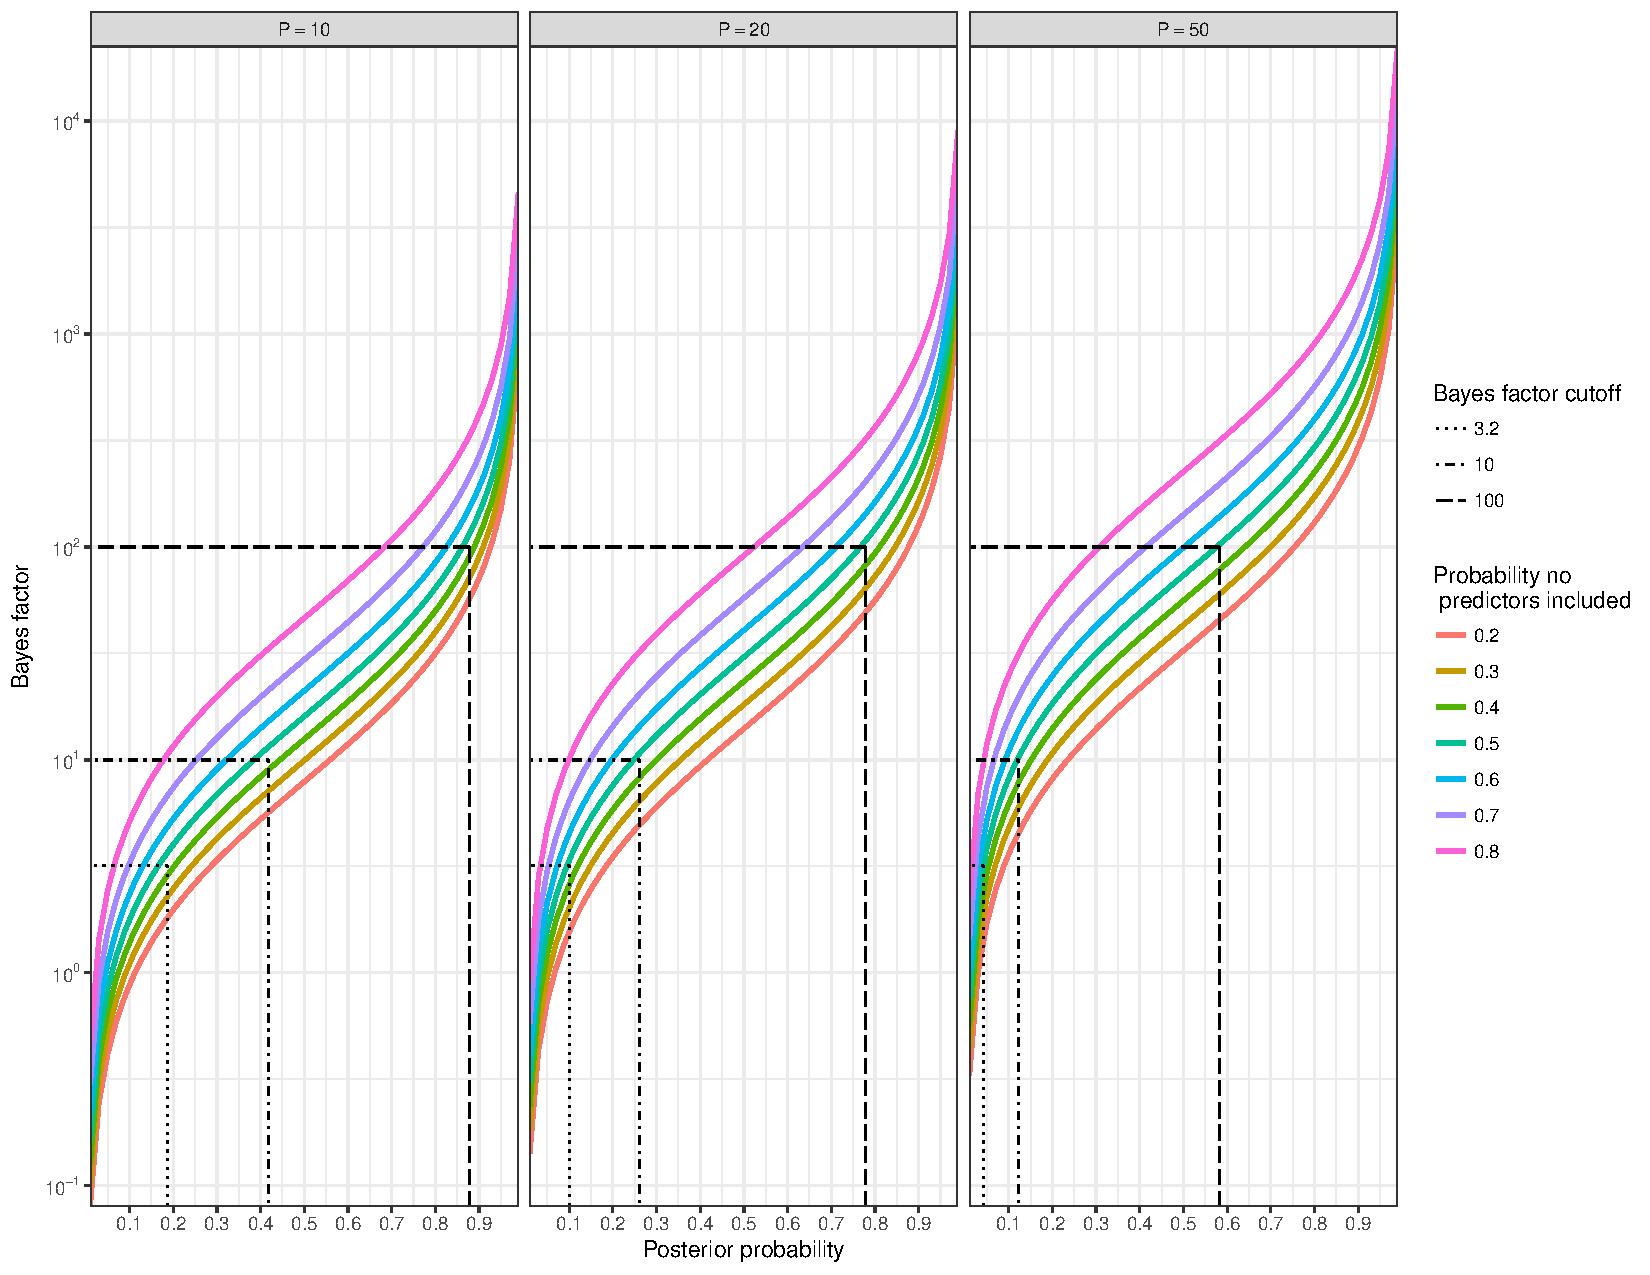
\includegraphics[width=1.15\textwidth]{\dir/figs/BF_cutoffs_BSSVS.pdf}
  \caption[Visualising the relationship between prior stringency and Bayes factors for SSVS]{\textbf{Visualising the relationship between prior stringency and Bayes factors for SSVS.}
  Here I show the relationship between the posterior inclusion probability of a covariate and the Bayes factor for various levels of stringency.
  I use dotted (dashed) lines to show three common levels of ``relevance'' of the Bayes factor as presented in~\cite{Kass1995} for the level of stringency adopted here ($w = 0.5$).
  The panels refer to the number of predictors ($P$) under consideration.
  Note how one needs to be careful about the calibration of $w$ as $P$ changes.
  }
  \label{fig:BFcalibration}
\end{figure}

\subsection{Modelling count data}
\label{sec:countmodelling}

Pertinent to the scientific questions addressed in this chapter is the issue of applying the model in~\ref{eq:eglm} to count data.
I now proceed to discuss some useful model extensions.

A natural choice in a GLM context is to assume that the data follow a Poisson distribution with mean $\lambda$, which implies a link function $g(\lambda) = \log(\lambda)$.
Hence one can devise a model of the form
\begin{align}
 \label{eq:poissonglm}
   Y_i &\sim \text{Poisson}(\lambda_i), \\
  \log(\lambda_i) &= \alpha + \sum_{k=1}^P \beta_k\delta_k X_{ki}.
\end{align}
This is a common and widely employed model for count data.
It may be the case however that $Var(\boldsymbol Y) >> E[\boldsymbol Y]$, i.e., that there is considerable \textbf{overdispersion} in the data.
Since under the Poisson distribution $ E[\boldsymbol Y] = Var(\boldsymbol Y) = \lambda$, this choice of model may prove too restrictive.
One way of accommodating overdispersion is the so-called ``observation-level random effects'' (ORLE) model, whereby an observation-specific error term is added~\citep{Hinde1982,Hill2007,Harrison2014}.
\begin{align}
 \label{eq:overdisppoissonglm}
   Y_i &\sim \text{Poisson}(\lambda_i), \\
  \log(\lambda_i) &= \alpha + \sum_{k=1}^P \beta_k\delta_k X_{ki} + \epsilon_i, \\
  \epsilon_i &\sim N(0, \sigma^2),
\end{align}
leading to a non-standard distribution for $\boldsymbol Y$ that has $E[\boldsymbol Y] =  \exp(\sigma^2/2)\lambda$ and $Var(\boldsymbol Y) = [\exp(2\sigma^2) - \exp(\sigma^2)] \lambda^2 + \exp(\sigma^2/2)\lambda$.
% , where $\mu = \boldsymbol X^\intercal \boldsymbol\beta$
When $\sigma^2 = 0 $, we recover the model in~\ref{eq:poissonglm}\footnote{I am keeping $\lambda$ consistent across parametrisations for ease of comparison.}.

An alternative approach to modelling overdispersion is to assume the data come from a negative binomial distribution:
\begin{align}
\label{eq:negbinglm}
 Y_i & \sim \text{NegBin}(p_i, r), \\
 p_i & = \frac{r}{(r + \lambda_i)},  \\ 
  \log(\lambda_i) &= \alpha + \sum_{k=1}^P \beta_k\delta_k X_{ki},
\end{align}
where $r$ is the over-dispersion parameter.
Under this model, $E[\boldsymbol Y] = \lambda$ and $Var(\boldsymbol Y) =  \lambda + \lambda^2/r$.
Note that $r$ for this model plays a similar role as $\sigma^2£$ for the model in~\ref{eq:overdisppoissonglm}.
The choice of model can be done on a generative basis, i.e., relative to the data-generating process or following model fit criteria (see below).

If the counts take place in space, for instance if we are modelling disease counts, a model that takes spatial -- and potentially temporal -- information into account could be specified.
Such a model is similar in structure to the ORLE model (\ref{eq:overdisppoissonglm}), with the addition of errors $\boldsymbol\eta$  that are not independent but assumed to follow some spatial process.
A common and flexible choice is the conditional autorregressive (CAR) model of Besag-York-Moill\'e (BYM)~\citep{Besag1991}:
\begin{align}
 \label{eq:bym}
   Y_i &\sim \text{Poisson}(\lambda_i), \\
  \log(\lambda_i) &= \alpha + \sum_{k=1}^P \beta_k\delta_k X_{ki} + \epsilon_i + \eta_i,
\end{align}
where the errors are assumed to have conditional distributions of the form
\begin{equation}
 \eta_i | \boldsymbol\eta_{-i} \sim \text{Normal}\left(\mu_i + \phi\sum_{i=1}^N\frac{W_{ij}}{D_{ii}}\left( \eta_j-\mu_j \right), \tau^2 D_{ii}^{-1} \right), 
\end{equation}
leading to the joint distribution
\begin{equation}
 \boldsymbol\eta \sim \text{Normal}\left(\boldsymbol\mu,  \tau^2 \left( \boldsymbol D - \phi \boldsymbol W \right)^{-1} \right),
\end{equation}
where $\boldsymbol W$ is a spatial weight matrix, usually $W_{ij} = 1$ if $i$ and $j$ are spatial neighbours and $W_{ij} = 0$ otherwise, with $W_{ii} = 0$.
A diagonal matrix $\boldsymbol D$ where $D_{ii} = \sum_{j = 1}^N W_{ij}$, a vector of means $\boldsymbol\mu$, a correlation parameter $\phi$ and a scale parameter $\tau$ complete the model specification.
A common simplification is to assume the spatial process has mean zero, i.e, $u_i = 0 \:\forall i$, since one is interested in describing the mean of the process using the covariates $\boldsymbol X$.
Here I consider only the so-called proper models, i.e., models for which  $|\phi| < 1$.
Data are usually not very informative with respect to $\phi$ and $\tau^2$, so it is customary to fix these parameters and then perform a sensitivity analysis to their fixed values.
I have implemented both the fully Bayesian version and the fixed parameter version, this latter having the advantage of much faster computation times.
For prior recommendations on the parameters of the models discussed in this section, I refer the viewer to~\cite{Gelman2006} for priors on the variance components and to~\cite[sec. 5.4.3]{Banerjee2003} for CAR model parameters.


Finally, I remark that it is usual when modelling disease data to write the mean as a product of an exposure variable $E_i$ and a relative risk, i.e., $\lambda_i = E_i e^{\psi_i}$.
An example of exposure variable would be the population in a certain area.

\subsection{Inference}
\label{sec:mcmc}

The (joint) posterior distribution for the parameters in~\ref{eq:eglm},
\[ p(\boldsymbol\theta| \boldsymbol X, \boldsymbol Y ) \propto f(\boldsymbol Y | \boldsymbol X, \boldsymbol\theta)\pi(\boldsymbol\theta), \]
where $\boldsymbol\theta = \{ \delta, \alpha, \sigma^2, \tau^2, ...\}$ stands for all parameters of interest, is not available analytically, but fortunately can be efficiently approximated using Markov chain Monte Carlo.
I implemented all models discussed in this chapter using the language JAGS~\citep{Plummer2003}.
% While very efficient Gibbs sampling schemes have been devised for the models considered here, I will instead take advantage of the Metropolis-Hastings machinery available in BEAST to sample the joint posterior of the parameters.
% To propose a new state $\boldsymbol\beta^\prime$, I will follow~\cite{Lemey2014} and draw $\boldsymbol\beta^\prime \sim \text{MVN}(\boldsymbol\beta, v \left( \boldsymbol X^\intercal \boldsymbol X\right)^{-1} )$, where $v$ is an adaptive parameter that can be used to tune the proposal so as to achieve a desired acceptance probability.
% Notice that this proposal scheme is only valid if the predictors are not collinear, i.e. if $\boldsymbol X^\intercal \boldsymbol X$ is invertible.
% To propose new values for the indicator variables $\boldsymbol\delta$ one can  employ a ``bit flip'' transition kernel.
% This transition kernel proposes a new value $\boldsymbol\delta^\prime$ by simply picking an element in $\boldsymbol\delta$ at random and ``flipping'' it, i.e., $\delta_j^\prime = 1$ if $\delta_j = 0$ and $\delta_j^\prime = 0$ otherwise.
% If one uses a different prior parametrisation, say places a prior on $S$ directly, $q(\boldsymbol\delta^\prime | \boldsymbol\delta)$ needs to be modified accordingly. 
% Please see Eq. 10 in~\cite{Drummond2010} for an example.
% To propose new values of the variance parameter $\sigma^2$ I employ a ``scale operator'' (see Chapter 1 for details).
I run  four independent chains for $M=50000$ iterations.
To draw inference about the model I then remove at least 10\% of the chain as burn-in and then use the resulting sample for all subsequent computations (calculating summaries, prediction, etc.).

Let $\mathbf{C}_j = \{ \delta_j^{(1)}, \delta_j^{(2)}, \ldots, \delta_j^{(M)} \} \in [0, 1]^M$ be a MCMC sample for the j-th indicator.
A natural choice of estimator for the posterior inclusion probability for the $j$-th covariate is $\hat{\delta_j} = (1/M)\sum_{k=1}^M \delta_j^{(k)}$.
Convergence was determined by visually inspecting the trace of all values in the chain and by computing effective sample sizes (ESS).
A chain was considered to have converged to the target distribution if all parameters had ESS$>200$.
When $\beta_j$ is close to zero the likelihood is nearly insensitive to whether $\delta_j = 0$ or $\delta_j = 1$, hence I monitor convergence of the product $\theta_j = \delta_j\beta_j$ instead, as advised by~\cite{OHara2009}.
% To provide a point of comparison, I also implemented this model in the popular probabilistic programming language \textbf{JAGS}~\citep{Plummer2003}.
Also of interest is the conditional distribution $p(\beta_j | \delta_j = 1)$, which I use to report coefficient estimates. 

Finally, from a Bayesian perspective prediction follows in a straightforward fashion from the posterior distribution:
\[ p(\boldsymbol Y_{new}  | \boldsymbol Y) = \int_{\Theta} p_1(\boldsymbol Y_{new} | \theta, \boldsymbol Y) p_2(\theta | \boldsymbol Y) d\theta.   \]
This means that one can simultaneously estimate parameters $\theta$  and compute predictions $\boldsymbol Y_{new}$ within the same chain in MCMC.

\subsection{Model comparison}
\label{sec:modcomp}

Between the choice of error distribution and the structure of the varying intercepts (random effects), there are a host of possible models one could build.
The issue of determining which model fits the data best is a central one in Statistics~\citep{Kass1995,Vehtari2017}.
Here I will employ two so-called information criteria to evaluate model fit, in addition to observed-versus-fitted analyses.
The first information criterion I consider is the deviance information criterion (DIC)~\citep{Spiegelhalter2002}.
Let $D(\boldsymbol\theta) = -2 \log(p(\boldsymbol Y | \boldsymbol\theta))$ be the model \textit{deviance}.
Then we define $\text{DIC} = E[D(\boldsymbol\theta)] + pD$, where the expectation is taken w.r.t the posterior and $pD$ is a model complexity penalty, calculated as in the commentary by Martyn Plummer in the discussion of~\cite{Spiegelhalter2002}.

A second information criterion I consider here is the  widely applicable information criterion (WAIC)~\citep{Watanabe2010}.
WAIC is constructed as a fully Bayesian model fit quantity, and takes into account the out-of-sample predictive power of the model.
WAIC is constructed as 
\[  \text{WAIC} = E[D(\boldsymbol\theta)] + 2\sum_{i=1}^N\left(\log E[p(Y_i | \boldsymbol \theta)] - E[\log p(Y_i | \boldsymbol \theta)] \right),\]
and has the major advantage of not relying on the existence of a ``true'' model.

In addition  to these univariate models of model fit, it is always prudent to assess model performance by evaluating its predictive power.
In particular, predicted versus fitted plots are quite helpful in determining how well a model reproduces the data it was fitted to.
By comparing prior and posterior predictive distributions for the data $\boldsymbol Y$ with its measured value one can gain insight not only into how well the model fits after data has been observed but also what sort of predictions the model generates using only the pre-data (i.e. prior) information.

\section{Modelling Ebola in West Africa}

In this section I describe the application of the modelling framework presented above to study the epidemic determinants of Ebola virus disease in West Africa.
Following the study by~\cite{Dudas2017} a rich set of socio-economic, climatic and genetic data was made available.
This chapter is concerned with exploring these data to gain further insight into the factors driving EBOV proliferation and persistence.

\subsection{Modelling case counts}

The first question of interest is modelling the relationship between the number of Ebola viral disease (EVD) cases and a plethora of socio-economic, climatic and genetic predictors.
Following~\cite{Dudas2017} I use administrative regions at the district (Sierra Leone), prefecture (Guinea) and county (Liberia) levels as the units of observation.
EVD case numbers are reported by the WHO for every country division (region) at the appropriate administrative level, split by epidemiological week.
I aggregate probable EVD cases and laboratory-confirmed cases in WHO reports\footnote{The main motivation for this approach is to -- partially -- accommodate subnotification.}.
This results in a data set with $81$ locations, $63$ of which reported one or more EVD cases.
The predictors available for this analysis are listed in Table~\ref{tab:predictorTable}.

I expand the case count analyses in~\cite{Dudas2017} in two ways.
Firstly, I include phylogenetic information in the form of the (average) number of predicted introductions, inferred from genetic data using a phylogeographic model.
I use the posterior average number of introductions into a certain region inferred from phylogenetic data using either presence/absence of administrative boundaries (\verb|VirIntroAdmin|) or distance  between locations (\verb|VirIntroDist|).
Details of how these computations were done are provided in the supplementary information of~\cite{Dudas2017}.


Secondly, I consider a setting with $57$ predictors whereas~\cite{Dudas2017} only considered $13$ predictors.
This leads to a classical $N < P$ situation, i.e,  a situation where one has as many  or more covariates/predictors as one has data points.
My goals are: (i) to investigate the association of predicted introductions and case numbers; (ii) to investigate some predictors not included in the original analysis and (iii) to predict how many cases would have occurred at the locations which reported zero EVD cases, i.e, the potential size of the epidemic in each location.

Pursuing goal (i) would allow me to assess the hypothesis that the EVD epidemic in West Africa was mainly driven by re-introductions whereas goal (ii) could not only lead to new insight into the driving factors behind the epidemic but also would allow me to investigate the power of BSSVS in a $N<P$ scenario.
Goal (iii) is important to assess the risk of new epidemics.

\begin{minipage}{\textwidth}  
\setcounter{mpfootnote}{\value{footnote}}
\renewcommand{\thempfootnote}{\arabic{mpfootnote}}
% \textsf{
\fontsize{9}{11}\selectfont
\begin{longtable}{ | l | l | p{.41\textwidth} | l | }
\caption{\textbf{Covariates considered for the case and persistence data modelling.} All continuous predictors were standardised by subtracting the mean and dividing by the sample standard deviation.}
\label{tab:predictorTable}\\
\hline
Predictor type & Abbreviation & Predictor description & Included\footnotemark[1]\\
\hline
Demographic & PopDens & Population density (inhabitants/Km$^2$) & yes\\ 
\hline
Demographic & TTXk & Estimated mean travel time in minutes to reach the nearest major settlement of at least X $\times$ 10,000 people, for X = 50, 100 and 500. & yes\\ 
\hline
Demographic & GrEconMN & Mean gridded economic output & yes\\ 
\hline
Demographic & GrEconMIN & Minimum gridded economic output & yes\\ 
\hline
Demographic & GrEconMAX & Maximum gridded economic output & yes\\ 
\hline
Demographic & GrEconSTD & Standard deviations of gridded economic output & yes \\ 
\hline
Demographic & LangX & Percentage of the population speaking language X, for $X = 1, 2, \ldots, 17$ & no\\ 
\hline
Climatic & AltMN & Mean altitude (elevation above sea level)& yes\\ 
\hline
Climatic & TempMN & Mean annual temperature & yes \\ 
\hline
Climatic & TempSSMN & Mean index of temperature seasonality & yes\\ 
\hline
Climatic & PrecipMN & Mean annual precipitation annual mean & yes\\ 
\hline
Climatic & PrecipSSMN & Mean annual seasonality in precipitation & yes\\ 
\hline
Climatic & PrecipX & Mean precipitation for month X, $X = 1, 2, \ldots, 12$ & no\\ 
\hline
Climatic & HumX & Mean humidity for month X, $X = 1, 2, \ldots, 12$ & no\\ 
\hline
Genetic & VirIntroAdmin & Mean number of viral introductions predicted using administrative borders & no\\ 
\hline
Genetic & VirIntroDist & Mean number of viral introductions predicted using distances between locations & no\\ 
\hline
Genetic & NumSeq & number of EBOV complete genome sequences collected & no\\ 
\hline
\end{longtable}
\footnotetext[1]{Whether the predictor was included in the original analysis in~\cite{Dudas2017}.}
\setcounter{footnote}{\value{mpfootnote}}
% }
\end{minipage}

\subsection*{EBOV persistence times}

A second outcome of interest is the persistence of EBOV and its determinants.
Combining genetic data and a phylogeographic model,~\cite{Dudas2017} computed the numbers of viral introductions from and to each location (where sequences were sampled) and then estimated the persistence times (in days) for each location.
Following the authors I define a cluster as a group of sequenced cases in a region that can be traced to a single introduction and then define persistence as the time from the MRCA and the last sampled sequence in the cluster.
For this data set, $N = 56$ data points were available, corresponding to the $56$ (admin 2 level) locations represented in the data analysed by~\cite{Dudas2017}. 

As with the analysis of case counts, my main goal is to ascertain which of the available predictors is strongly associated with viral persistence in a given region.
Since persistence times are a continuous, strictly positive outcome, I chose the log-normal and Gamma family of distributions to model its variation.
The hierarchical model presented in~\ref{eq:bym}, for instance, can be extended to any exponential family distribution, as shown in~\cite[Sec. 5.5]{Banerjee2003}.
For these analyses I included the number of sequences per location (\verb|NumSeq|) and the (standardised) population size (\verb|PopSize|) as predictors.
This is important as the number of sequences sampled in a given location control the ``sample size'' from which persistence times are computed.
The more sequences sampled in a region, the more tips will be available to compute persistence times.
In the same fashion as the analyses of case counts, I also consider an additional situation where a larger number of predictors are available ($P = 58$, $N = 56$).
 
\section{Results and discussion}

In what follows I present the results of fitting 10 models to each data set in fully Bayesian fashion from which I compute Bayes factors and extract (posterior) predictions.
I employ the Bayes factors from SSVS to tease apart which factors are associated with the outcome of interest and use posterior predictions for the regions with no reported cases (case data) or no sequences (persistence data) as a way o gaining insight into a region's potential for sustaining transmission chains in both size and duration.


For the EVD case data, Table~\ref{tab:casesModels} shows that a Poisson model with (unstructured) observation-level ``random effects'' (OLRE, model 2) showed best performance in terms of fit and hence I chose its SVSS counterpart, model 7, as the basis for computing Bayes factors for the predictors.

\begin{minipage}{\textwidth}    
\setcounter{mpfootnote}{\value{footnote}}
\renewcommand{\thempfootnote}{\arabic{mpfootnote}}
\fontsize{9}{10}\selectfont
\rowcolors{5}{gray!25}{white}
\begin{longtable}{cccccccc}
\caption{\textbf{Modelling results for EVD case data.}
% Taking fit (WAIC and DIC) and predictive performance into account, I elect model 7 as the best model and use it in all further analyses.
}
\label{tab:casesModels}\\
\toprule
Model & Distribution & Intercept& Variable inclusion & DIC  & WAIC   & RMSE\footnotemark[1] & Obs. in CI\footnotemark[2]\\
\toprule
0  & Poisson & Single intercept & Full & 5204  & 8717.3 & 1.83$\times 10^2$ & 15\\
\hline
1   & Negative Binomial & Single intercept & Full & 738.8 & 731.4  & 2.15$\times 10^4$& 62\\
\hline
2 & Poisson & OLRE & Full & 489   & \textbf{476.4} & \textbf{0.73} & 63\\
\hline
3 & Poisson & OLRE/spatial\footnotemark[3] & Full & 481.5 & 478.1  & 0.84 & 63 \\
\hline
4 & Negative Binomial & OLRE/spatial\footnotemark[4] & Full & 737.9 & 731.4 & 2.14$\times 10^4$ & 63\\
\hline
5 & Poisson  & Single intercept & SSVS & 5181  & 8492.9 & 1.85$\times 10^2$ & 14\\
\hline
6 & Negative Binomial & Single intercept & SSVS & 763.6 & 747.2  & 7.38$\times 10^2$& 63\\
\hline
7 & Poisson & OLRE & SSVS & 490.9 & 478.3  & 0.76   & 63\\
\hline
8 & Poisson & OLRE/spatial\footnotemark[3] & SSVS & \textbf{475.8} & 477.4  & 1.14 & 63\\
\hline
9 & Negative Binomial & OLRE/spatial\footnotemark[4]& SSVS & 758.2 & 747.6 & 6.49$\times 10^2$ & 63\\
\bottomrule
\end{longtable}
\footnotetext[1]{Root mean squared error, $\sqrt{\sum_{i=1}^N \left(Y_i-\hat{Y_i} \right)^2/ N}$.}
\footnotetext[2]{Number of observations -- out of $N=63$ -- within the predicted 95\% credibility interval (CI).}
\footnotetext[3]{This is the BYM model as in~\ref{eq:bym}.}
\footnotetext[4]{These models do not have the ORLE component.}
\setcounter{footnote}{\value{mpfootnote}}
\end{minipage}

In a similar fashion, in Table~\ref{tab:persistenceModels} I present the results of fitting 10 models to the persistence time data described above.
Results point model 2 (log-normal OLRE) as the best performing model.
However, the SSVS counterpart to model 2, model 7, shows worse performance when compared with model 8, which includes a spatial component.
I thus decide to use model 8 for all further investigations.

\begin{minipage}{\textwidth}    
\setcounter{mpfootnote}{\value{footnote}}
\renewcommand{\thempfootnote}{\arabic{mpfootnote}}
\fontsize{9}{10}\selectfont
\rowcolors{5}{gray!25}{white}
\begin{longtable}{cccccccc}
\caption{\textbf{Modelling results for EVD persistence times.}}
\label{tab:persistenceModels}\\
\toprule
% \rowcolor{gray!50}
Model & Distribution & Intercept& Variable inclusion & DIC  & WAIC   & RMSE\footnotemark[1] & Obs. in CI\footnotemark[2]\\
\toprule
0  & Log-normal & Single intercept & Full & 495.9 & 502.7 & 12932.85 & 55 \\
\hline
1   & Gamma & Single intercept & Full &  507.1 & 489.6 & 14739.0 & 54 \\
\hline
2 & Log-normal & OLRE & Full &  \textbf{428.5} & \textbf{329.1} & 142.6   & 56 \\
\hline
3 & Log-normal & OLRE/spatial\footnotemark[3] & Full & 508.8 & 362.9 & 198.3   & 56 \\
\hline
4 & Gamma & OLRE/spatial\footnotemark[4] & Full & 483.8 & 489 & 9889.6  & 56 \\
\hline
% \midrule
5 & Log-normal  & Single intercept & SSVS & 496.7 & 494.5 & 19838.0 & 54 \\
\hline
6 & Gamma & Single intercept & SSVS & 487.8 & 486.1 & 19480.4 & 53 \\
\hline
7 & Log-normal & OLRE & SSVS &  496.8 & 377.4 & 360.5 & 56 \\
\hline
8 & Log-normal & OLRE/spatial\footnotemark[3] & SSVS & 452.2 & 330.2 & \textbf{51.6}  & 56 \\
\hline
9 & Gamma & OLRE/spatial\footnotemark[4]& SSVS &  491.3 & 488.6 & 14554.1 & 55 \\
\bottomrule
\end{longtable}
\footnotetext[1]{Root mean squared error, $\sqrt{\sum_{i=1}^N \left(Y_i-\hat{Y_i} \right)^2/ N}$.}
\footnotetext[2]{Number of observations -- out of $N=56$ -- within the predicted 95\% credibility interval (CI).}
\footnotetext[3]{This is a modified BYM model (\ref{eq:bym}) to accommodate different error distributions.}
\footnotetext[4]{These models do not have the ORLE component.}
\setcounter{footnote}{\value{mpfootnote}}
\end{minipage}

\subsection*{Epidemiological findings}

I use the models to answer to major questions emerging from the 2013-2016 West African EVD epidemic: (i) what drove the local proliferation of transmission chains (cases) and (ii) which factors were associated with viral persistence in a given region.

\subsection*{What are the driving factors behind EBOV proliferation and persistence?}

Using model 7 in Table~\ref{tab:casesModels}, I computed the Bayes factors for all $P = 15$ predictors and keep those that show ``strong evidence'' according to~\cite{Kass1995} ($\text{BF}>3$), presented in Table~\ref{tab:case_glm_results}.
In agreement with findings of~\cite{Dudas2017}\footnote{See Table 2 therein for comparison.}, the predictors strongly associated with case counts are environmental factors such as temperature seasonality, precipitation and temperature.
Additionally, travel time to the nearest 50 and 100 thousand inhabitants settlement, which are socio-economic variables that reflect a region's connectedness, also had higher Bayes factors.
It should be noted that the results presented here differ from the ones in~\cite{Dudas2017} in that the authors chose to include population sizes as a covariate, whereas I opt to use population sizes as an exposure variable and thus model relative rates.

Importantly, the genetic covariates relating to the numbers of viral introductions (\verb|VirIntroAdmin| and \verb|VirIntroDist|) were not strongly associated with case counts.
This is a puzzling result, since all the evidence points towards the fact that the 2013-2016 EVD epidemic was mainly driven by migration of infected individuals (i.e., a ``sparks and fires'' model).
It is possible that these variables were in fact poor proxies for the actual numbers of viral introductions into a given region.
I deliberately chose these two variables because they did not include any ``gravity'' information, that is information about population sizes.
This was to avoid correlation between the covariates and the exposure variable.
It remains to be seem whether a better measure of viral introductions would help explain case counts.
Another possibility is a complex interplay between the number of introductions a region receives and the local conditions (environmental, socio-economic, cultural) that cannot be captured by a linear model.

\begin{minipage}{\textwidth}    
\setcounter{mpfootnote}{\value{footnote}}
\renewcommand{\thempfootnote}{\arabic{mpfootnote}}
% \textsf{
\fontsize{9}{11}\selectfont
\rowcolors{5}{gray!25}{white}
\begin{longtable}{lcccc}
\caption{\textbf{Variable selection for the EVD case data.}
I present the results from model 7 (see Table~\ref{tab:casesModels}).
}
\label{tab:case_glm_results}\\
\toprule
Predictor\footnotemark[1] & Coefficient\footnotemark[2] & 95\% CI\footnotemark[3] & Inclusion\footnotemark[4] & BF\footnotemark[5] \\
\toprule
TempSSMN & -1.52 & -2.17, -0.70 & 0.82 & 99.6 \\
\hline
PrecipMN & 1.15 & 0.35, 1.91 & 0.35 & 11.6 \\
\hline
TT50K &  -0.71 & -1.21, -0.27 & 0.31 & 9.4 \\
\hline
TempMN &  0.63 & 0.18, 1.08 & 0.20 & 5.4 \\
\hline
TT100K & -0.59 & -1.11, 0.64 & 0.17 & 4.2\\
\bottomrule
\end{longtable}
\footnotetext[1]{Predictors with Bayes factor $>$3.}
\footnotetext[2]{Posterior mean of the coefficient.}
\footnotetext[3]{95\% posterior credible interval (CI).}
\footnotetext[4]{Posterior inclusion probability for the predictor.}
\footnotetext[5]{Bayes factor (BF).}
% }
\setcounter{footnote}{\value{mpfootnote}}
\end{minipage}

I extend the analyses in~\cite{Dudas2017} by considering a much larger set of predictors ($P = 57$, description in Table~\ref{tab:predictorTable}), taking advantage of the SSVS framework.
Results in Table~\ref{tab:case_bigP_results} are wholly consistent with the previous results, with most of the selected covariates being environmental variables related to precipitation, humidity and temperature.
An important exception is the inclusion of the variable \verb|Lang4| which measures the percent of speakers of { \color{red}{SOME LANGUAGE} } in a region.
This is a variable that was not considered by~\cite{Dudas2017} and its inclusion with high probability indicates that cultural factors might shape local transmissibility conditions (see~\cite{Alexander2015} and references therein).
Further investigation is needed before more elaborate hypotheses can be formulated.

\begin{minipage}{\textwidth}    
\setcounter{mpfootnote}{\value{footnote}}
\renewcommand{\thempfootnote}{\arabic{mpfootnote}}
% \textsf{
\fontsize{9}{11}\selectfont
\rowcolors{5}{gray!25}{white}
\begin{longtable}{lcccc}
\caption{\textbf{Variable selection for the EVD case data with $P = 57$ predictors.}
As with the results in Table~\ref{tab:case_glm_results}, I present the results from model 7 and include all covariates with Bayes factor larger than 3.} 
\label{tab:case_bigP_results}\\
\toprule
Predictor\footnotemark[1] & Coefficient\footnotemark[2] & 95\% CI\footnotemark[3] & Inclusion\footnotemark[4] & BF\footnotemark[5] \\
\toprule
Lang4 & -1.12 & -1.66, -0.61 & 0.66 & 153.9 \\
\hline
Pre10MN & 1.05 & 0.63, 1.58 & 0.53 & 91.2 \\
\hline
Pre08MN & 1.45 & 0.70, 2.12 & 0.27 & 30.2 \\
\hline
pre04MN & 1.54 & 0.72, 2.04 & 0.23 & 23.6 \\
\hline
Hum08MN & 1.04 & 0.35, 1.60 & 0.14 & 12.8 \\
\hline
Pre09MN & 1.04 & 0.43, 2.02 & 0.12 & 11.1 \\
\hline
Hum04MN & -1.43 & -2.94, -0.43 & 0.08 & 7.0 \\
\hline
Pre11MN & 0.90 & 0.15, 1.57 & 0.04 & 3.0 \\
\hline
PrecMN & 1.46 & 0.37, 2.20 & 0.04 & 3.0 \\
\hline
Hum05MN & -1.14 & -2.83, -0.11 & 0.04 & 3.0 \\
\hline
TempMN & -0.64 & -1.09, -0.23 & 0.03 & 3.0 \\
\hline
PrecssMN & -1.26 & -2.03, 0.16 & 0.03 & 3.0 \\
\bottomrule
\end{longtable}
\footnotetext[1]{Predictors with Bayes factor $>$3.}
\footnotetext[2]{Posterior mean of the coefficient.}
\footnotetext[3]{95\% posterior credible interval (CI).}
\footnotetext[4]{Posterior inclusion probability for the predictor.}
\footnotetext[5]{Bayes factor (BF).}
% }
\setcounter{footnote}{\value{mpfootnote}}
\end{minipage}

When looking at persistence times and considering $P = 15$ predictors, the only predictor with a strong association with the outcome was the number of sequences in a region (Table~\ref{tab:persistence_glm_results}), which was included as a control variable.
Because of how the persistence times are computed, one expects them to be positively correlated with the number of sequences, hence this result is unsurprising.
On the other hand, lack of association with any of the other of variables is itself informative insofar as it suggests that we might not be  able to explain viral persistence by considering solely local factors.

\begin{minipage}{\textwidth}    
\setcounter{mpfootnote}{\value{footnote}}
\renewcommand{\thempfootnote}{\arabic{mpfootnote}}
% \textsf{
\fontsize{9}{11}\selectfont
\rowcolors{5}{gray!25}{white}
\begin{longtable}{lcccc}
\caption{\textbf{Variable selection for persistence time data.}
I present the results from model 8 (see Table~\ref{tab:persistenceModels}).}
\label{tab:persistence_glm_results}\\
\toprule
Predictor\footnotemark[1] & Coefficient\footnotemark[2] & 95\% CI\footnotemark[3] & Inclusion\footnotemark[4] & BF\footnotemark[5] \\
\toprule
Sequence count & 0.19 & 0.08, 0.33 & 0.21 & 5.77 \\
\bottomrule
\end{longtable}
\footnotetext[1]{Predictors with Bayes factor $>$3.}
\footnotetext[2]{Posterior mean of the coefficient.}
\footnotetext[3]{95\% posterior credible interval (CI).}
\footnotetext[4]{Posterior inclusion probability for the predictor.}
\footnotetext[5]{Bayes factor (BF).}
% }
\setcounter{footnote}{\value{mpfootnote}}
\end{minipage}

I refine my analysis by considering a larger set of $P = 58$ covariates and find that, in addition to sequence counts as before, only one more variable shows substantial association with persistence times (Table~\ref{tab:persistence_bigP_results}).
The variable \verb|Precip01|, which measures the average precipitation in January in a given region, was included with high probability.
This result is hard to explain since there is no obvious link between the amount of rain in a particular month and favourable conditions for viral lineage persistence.
Interestingly, (standardised) population sizes failed to attain a high inclusion probability in any of the SSVS models, suggesting that, somewhat counterintuitively, how big the population is in a given area does not significantly impact its suitability for persisting lineages. 

\begin{minipage}{\textwidth}    
\setcounter{mpfootnote}{\value{footnote}}
\renewcommand{\thempfootnote}{\arabic{mpfootnote}}
% \textsf{
\fontsize{9}{11}\selectfont
\rowcolors{5}{gray!25}{white}
\begin{longtable}{lcccc}
\caption{\textbf{Variable selection for persistence time data with $P = 58$ predictors.}
I present the results from model 8 (see Table~\ref{tab:persistenceModels}).}
\label{tab:persistence_bigP_results}\\
\toprule
Predictor\footnotemark[1] & Coefficient\footnotemark[2] & 95\% CI\footnotemark[3] & Inclusion\footnotemark[4] & BF\footnotemark[5] \\
\toprule
Precip01 & -0.35 & -0.51, -0.16 & 0.11 & 10.0 \\
\hline
Sequence count & 0.20 & 0.07, 0.31 & 0.06 & 5.2\\
\bottomrule
\end{longtable}
\footnotetext[1]{Predictors with Bayes factor $>$3.}
\footnotetext[2]{Posterior mean of the coefficient.}
\footnotetext[3]{95\% posterior credible interval (CI).}
\footnotetext[4]{Posterior inclusion probability for the predictor.}
\footnotetext[5]{Bayes factor (BF).}
% }
\setcounter{footnote}{\value{mpfootnote}}
\end{minipage}

\subsection*{Why did the epidemic not spread further?}

Whether a epidemic develops in a region depends on multiple factors, mainly (i) whether the virus is introduced with high frequency and (ii) the local conditions are favourable for maintenance of sustained transmission chains.
While this chapter is mainly concerned with (ii), a complete picture of the epidemic can only be painted by also including (i).
While I tried to address (i) by including the variables \verb|VirIntroAdmin| and \verb|VirIntroDist|, I now focus on (ii) with the hope of gaining insight into why some regions did not experience EVD cases.

Figure~\ref{fig:mapsCases} shows the observed and predicted numbers of EVD cases and also the incidence per 100, 000 inhabitants.
This is important because even though the absolute number of cases is an important epidemiological variable, incidence rates provide a relative (scaled) measure of the disease burden in a given region.
Using a Poisson model with OLRE and SSVS (mode 7, Table~\ref{tab:case_glm_results}), I predict that Cavally and Tonkpi (in the Ivory Coast) for instance would have experienced $470$ (1, 2547) and $1225$ (0, 8854) cases, respectively.
Despite these numbers being reasonably high compared to the overall average of 387 (95\% credible interval: 2, 2206), they would mean incidences of 111 and 129 cases per 100, 000 inhabitants, which are not substantially high compared to the average of 97 (2, 408) cases/100K.
These are predictions the epidemic potential, however, as these regions did not report any cases.
This suggests that while local conditions were conducive to the development of epidemics, the number of introductions into these locations, among other factors, was not enough to lead to successful establishment of transmission chains. 

\begin{figure}[htbp]
  \centering
  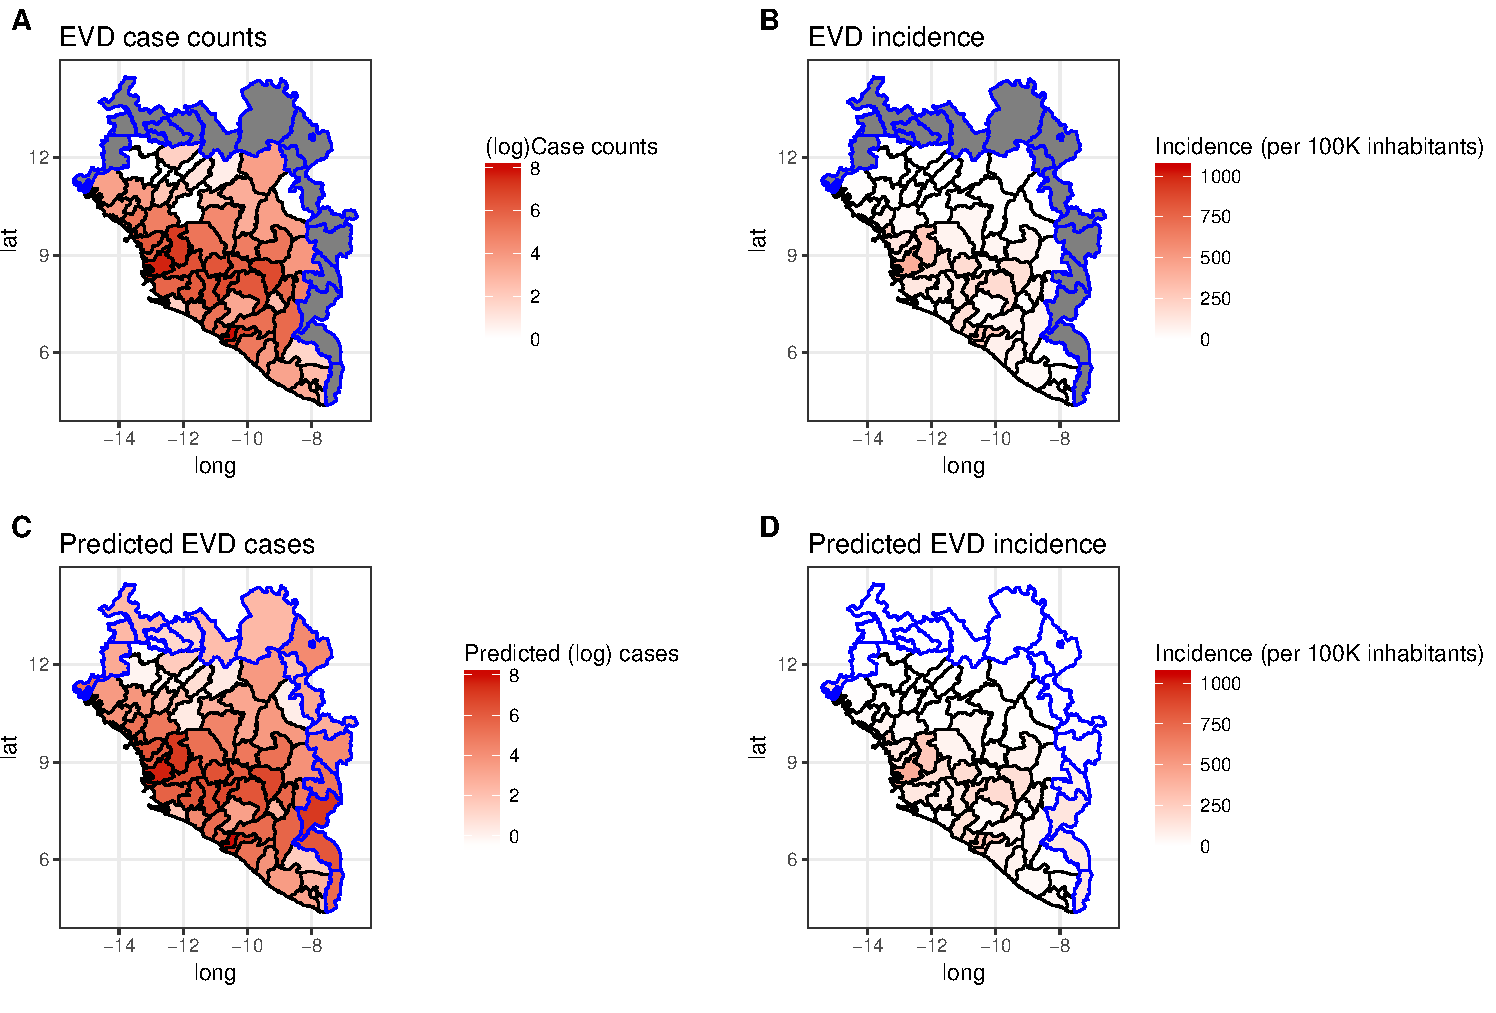
\includegraphics[scale=0.65]{\dir/figs/maps_cases_model7.pdf}
  \caption[Case counts predictions]{\textbf{Posterior means for the numbers of EVD cases and incidence.}
  Shaded areas show locations for which no cases were reported.
  Results from the Poisson model with observation-level varying intercepts (``OLRE'') and SSVS (model 7) show reasonable in-sample predictive ability.
  Regions such as Tonkpi were predicted to have moderate EVD incidence despite being predicted to have higher than average numbers of EVD cases.
  }
  \label{fig:mapsCases}
\end{figure}

When considering predictions for persistence times, I show results for models 2 and 8 (see Table~\ref{tab:persistenceModels} for details).
In order to identify areas with a particularly higher suitability for persistence, I select the locations with predicted values in excess of the 75\% percentile of the predictive distribution of persistence times.
Predictions from model 2 showed that Kenieba (Mali), Saraya, Tambacounda, Velingara (Senegal) were above the threshold.
Using a log-normal distribution with OLRE and spatial structure (model 8), the locations Bafing, Kabadougou, San Pedro (Ivory Coast), Kedougou, Salemata, Velingara (Senegal), Tombali, Gabu (Guinea-Bissau), Kenieba, Kati, Kangaba and Yanfolila (Mali) were all predicted to be above the 75\% percentile.
As with the case counts, the predictions seemed to reflect the pattern of the observed data quite well (Figure~\ref{fig:mapsPersistence}).
Interestingly, none of these locations were predicted to have high numbers of cases.
This result is consistent with the findings in Tables~\ref{tab:case_glm_results},~\ref{tab:case_bigP_results},~\ref{tab:persistence_glm_results} and~\ref{tab:persistence_bigP_results}, that showed almost no overlap between the factors associated with EVD case numbers and persistence times.

\begin{figure}[htbp]
  \centering
  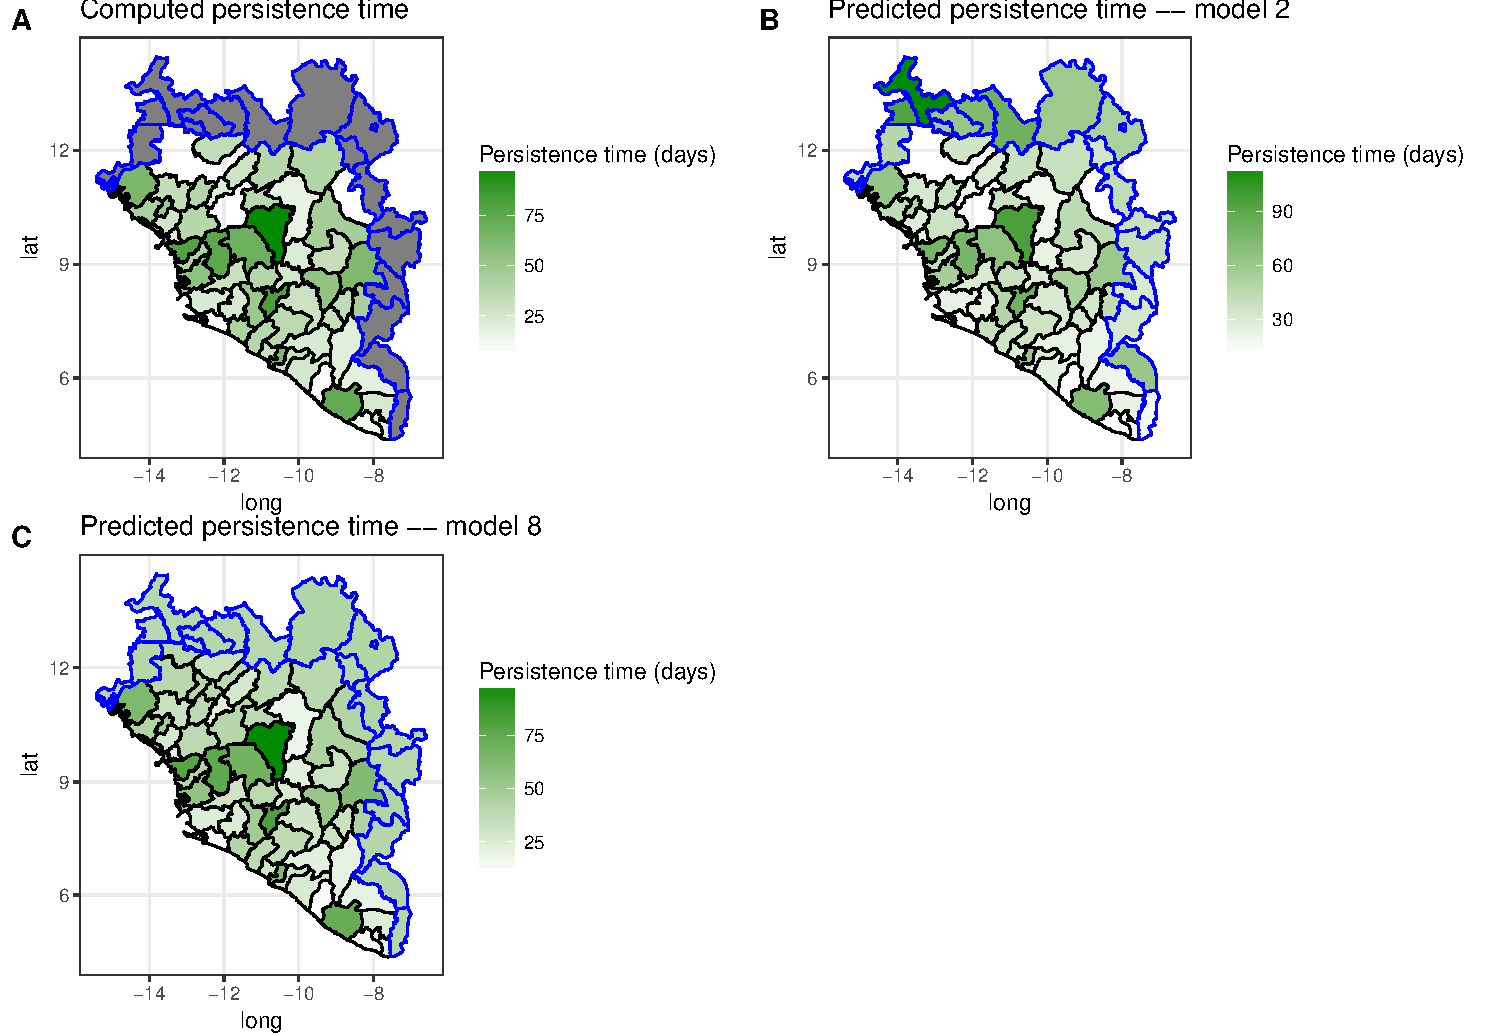
\includegraphics[scale=0.65]{\dir/figs/maps_persistence_model2_model8.pdf}
  \caption[Persistence times predictions]{\textbf{Posterior means of the computed by~\cite{Dudas2017} and predicted EBOV persistence times (in days).}
  I present predictions from models $2$ and $8$ (see Table~\ref{tab:persistenceModels}).
  }
  \label{fig:mapsPersistence}
\end{figure}


In short, the lack of overlap between the regions that were predicted to have higher numbers of cases and those predicted to have higher persistence times might help explain why the epidemic did not spread into these regions.
The role of border closure and other control measures should not be disregarded, however.
See~\cite{Dellicour2017} for an interesting follow-up paper employing phylodynamic methods to address which interventions would have been effective in curbing the epidemic in West Africa.
The complex interplay between migration of infected individuals between locations and the local ``suitability'' of each region is evidenced by the lack of clear spatial structure (see discussion on spatial models below).
Complex patterns of migration of infected individuals -- over long distances for instance -- and border closure mean that two areas that are geographic neighbours would have very different epidemic dynamics, hence leading to a situation with low spatial autocorrelation.


Hence, in summary:
\begin{itemize}
 \item Some regions that report no EVD cases were  predicted to have high epidemic potential;
 \item Several regions in Mali and Senegal were predicted to have higher suitability for viral persistence;
 \item The lack of overlap between areas with high predicted numbers of cases and persistence times can explain why the epidemic did not spread further.
\end{itemize}


\subsection*{Methodological findings}

I now focus on the technical aspects of the modelling effort presented in this chapter.
I would like to point out that while I lay out a complete framework for modelling epidemiological data in this chapter, I make no claims of originality.
See the frameworks proposed by e.g.~\cite{Scheel2013} and~\cite{Boehm2015} which touch on the same ideas explored in this chapter: generalised linear models, spatial structures and variable selection.

A first question one might ask is whether including an explicit spatial component improves model fit and (predictive) performance.
To assess the amount of variation that is structured spatially, one can compute $\gamma = \text{sd}(\boldsymbol\eta)/\left(\text{sd}(\boldsymbol\eta)  +  \text{sd}(\boldsymbol\epsilon)\right)$.
The closer $\gamma$ is to $1$ the more spatial structure there is in the data.
For all of the models considered here including both data sets (cases and persistence) $\gamma$ was estimated in the range $0.40 - 0.60$ with substantially wide credibility intervals.
This points decisively in the direction of the \textbf{absence} of appreciable (residual) spatial structure.

In keeping with these results, I find that models that include an spatial component perform no substantially better than models that include an unstructured, observation-level error term (see RMSE in Tables~\ref{tab:casesModels} and~\ref{tab:persistenceModels}).
In general, Poisson models with OLRE, whether an explicit spatial component was present or not (i.e., models $2$, $3$ $7$ and $8$) presented better fit and predictive performance.
From a methodological standpoint, one could argue that adding a spatially-varying error term might lead to overfitting when no extra-Poisson variation exists, but this has been shown to be a minor concern unless there is very strong spatial autocorrelation~\citep{Latouche2007}.
An attentive reader will notice I do not include an ORLE term in the negative binomial (cases) and Gamma (persistence) models.
This is to avoid parameter identifiability issues between the ORLE variance $\sigma^2$ and the overdispersion ($r$) and shape ($k$) parameters respectively.


A second question that may arise is whether employing BSSVS to select parsimonious models significantly reduces model fit and predictive performance.
Overall, results show that models where all covariates are included (``Full'') had better fit and predictive performance.
This pattern was consistent between the models for cases and persistence times -- hence 10 pairs of model comparisons.
However, these differences were not particularly marked.
In addition, while the analyses with many predictors ($P \geq N$) helped refine our understanding of the factors associated with both epidemic potential (cases) and viral persistence, I observed no gain in predictive performance for any of the 10 models\footnote{For each data set, there were five models with SSVS.} considered.
This result is not entirely surprising, since while including more predictors should increase the amount of data variation explained by the model, in a Bayesian setting it also means incorporating uncertainty about all the  extra parameters.

The BSSVS framework employed here has two major strengths.
On one hand it allows one to analytically compute Bayes factors for predictors and thus formally assess the relevance of the association between predictor and outcome of interest.
On the other, prior modelling is straightforward insofar as stringency/parsimony is concerned (see Figure~\ref{fig:BFcalibration}).
I note that whilst we make the assumptions of (prior) independence and exchangeability  in order to greatly simplify calculations and implementation, it is possible to explicitly include dependencies between predictors~\citep{Chipman1996}.
Unfortunately, and perhaps witness to the plethora of variable selection methods currently available, BSSVS also has major flaws that limit its applicability.
One such flaw is almost obvious to the trained  eye: because of multicolinearity between covariates, we expect models that include either variable from a pair of highly correlated covariates to be about equally as probable.
This rationale can be extended to see that several models amongst the $2^P$ possible will have virtually the same posterior mass. 
One could attempt to circumvent this fundamental multimodality by careful prior modelling, but this is not pursued further in this chapter. 

Finally, I would like to add a note about prior calibration for the class of models considered here.
It is clear from the prior predictive analyses that the usually recommended priors on the coefficients and other parameters induce a prior on the data $\boldsymbol Y$ that is miscalibrated.
For all the models considered for both data sets, sampling from $\pi(\boldsymbol\theta)$ led to an induced distribution  on $\boldsymbol Y$ that was more than 10 orders of magnitude off.
Unfortunately, a complete prior calibration study is outside the scope of this chapter, but remains an open avenue for future research.
% 
The statistical findings can be summarised as:
\begin{itemize}
 \item Variable selection was robust to choice of error distribution (Poisson/negative binomial \& Gamma/log-normal);
 \item There is very low residual spatial autocorrelation in the data, leading to unstructured models (OLRE) providing better fit;
 \item Current state-of-the-art recommended priors for the BYM model lead to a miscalibrated induced distribution on the data $\boldsymbol Y$.
\end{itemize}


\section{Conclusions and perspectives}

In this chapter I have presented a complete statistical framework to study the association of climatic, socio-economic and genetic predictors with EVD cases and EBOV persistence.
I extend the analyses presented in~\cite{Dudas2017} for the EVD case data by including the predicted number of viral introductions into each region, and further refine their results by exploiting BSSVS to include a large number of predictors and compute their Bayes factors.
Using the posterior predictive distribution, I study which regions that reported no EVD cases would be at higher risk of experiencing epidemics.
The modelling of persistence times is the missing piece from~\cite{Dudas2017}, who looked at case counts alone.
I employ the framework presented here to investigate the association of several predictors with viral persistence and also perform predictions in the same fashion as above.
I combine the predictions for case counts and viral persistence times to show very little overlap between areas with high epidemic potential and areas with increased suitability for viral persistence.
Since both these factors need to be in place for an outbreak to develop, I argue that these results partially explain why many areas did not report EVD outbreaks even though many of their spatial neighbours experienced widespread epidemics.

Phylodynamic methods allow us to extract epidemiological information from genomic data that would otherwise not be available \textit{via} traditional epidemiological methods.
Phylogeography in particular allows for inferences about the latent process of disease spatial spread as infected individuals move in space and then infect others.
For the first time we had a rich, densely-sampled, genomic data set that revealed the migration-driven nature of the Ebola epidemic in West Africa, which in practice meant that areas that are neighbours in geographical space need not be strongly connected, whilst areas separated by hundreds of kilometres might be epidemiologically linked.
This chapter contains an interesting complementary finding, with implications for disease spatial modelling.
None of the spatial models employed here showed better fit to the data, and the fraction of unexplained variation that is spatially structured was small.
These results suggest that future disease mapping efforts might greatly benefit from incorporating phylogeographic data in their prior specification.
One such way of incorporating migration information is to re-define a neighbourhood structure based not on geographic proximity or sharing of borders but on the viral flow between two regions.
Exactly how to incorporate this information and what effect this will have in the fitted models remains an open avenue of future research.

Whilst joint modelling of phylogeny and epidemiology remains the ultimate goal, I show that a principled statistical analysis of phylodynamic data (output) can also provide valuable biological insight -- see chapter 7 for a more general discussion on the value of separate analysis of phylodynamic data.
Traditional epidemiological techniques, when supplemented by phylogenetic/phylodynamic analyses, can lead to a better understanding of the processes shaping pathogen spread within and between populations.
